\documentclass[relatorio,oneside]{iagtese}	       % subclasse relatorio do iagtese
										%
%\documentclass[relatorio,oneside]{iagtese_en}	% subclasse relatorio do iagtese
										% em ingles. Para escrever o
										% relatorio em ingles, descomente
 										% esta linha e comente a linha
                                            					% anterior.
\def\today{Agosto de 2020 a Março de 2021 }% período a que se refere o relatório
										%
										%
\begin{document}							% início do documento
										%
\institution{Universidade de S�o Paulo \\ Instituto de Astronomia, Geof�sica e Ci�ncias Atmosf�ricas \\ Departamento de Astronomia}

\title{T�tulo do trabalho}

\translator{{Tese/Disserta��o apresentada ao Departamento de Astronomia do Instituto de Astronomia, Geof�sica e Ci�ncias Atmosf�ricas da Universidade de S�o Paulo como requisito parcial para a obten��o do t�tulo de Mestre/{}Doutor em Ci�ncias.\\ \\
�rea de Concentra��o: Astronomia\\
Orientador(a): Prof.($^{\rm a}$) Dr.($^{\rm a}$) Orientador(a)}}

\author{Autor}

\date{S�o Paulo \ano}
							% arquivo para inserir a capa
										%
%% \titulo									%
										%
\assinatura								% folha com assinaturas

%% % Autor: Gabriel Góes Rocha de Lima
% Descrição: Resumo do postesr para o II workshop Inteligência Artificial e Geociências

\documentclass[11pt]{article} % declaração do tipo de documento
\usepackage[utf8]{inputenc} % declaração do tipo de codificação
\usepackage{geometry} % pacote para definição de margens
\usepackage{ragged2e} % Texto justificado
\usepackage{indentfirst} % pacote para indentação do primeiro parágrafo
\usepackage{setspace} % pacote para definição de espaçamento
\usepackage{titlesec} % Pacote para formatação de títulos

\geometry{a4paper, left=2cm, right=2cm, top=2cm, bottom=2cm} % definição das margens
\onehalfspacing % espaçamento de 1.5
\setlength{\parindent}{1.25cm} % indentação de 1.25cm
\setlength{\parskip}{0.5em} % set distance spacing between paragraphs
%\renewcommand{\baselinestretch}{1.5} % set line spacing
%\setmainfont{SourceCodePro Nerd Font} % Definindo a fonte principal
\titleformat{\section}{\normalfont\bfseries}{\thesection}{1em}{} % Formatação de títulos de seção
\titleformat{\subsection}{\normalfont\bfseries}{\thesubsection}{1em}{} % Formatação de títulos de subseção


\begin{document} % início do documento
\title{Da Terra ao Código: Integrando Dados Geológicos com Inteligência Computacional} % título do documento
\author{Gabriel Góes Rocha de Lima} % autor do documento
\date{28 de fevereiro de 2024} % data do documento
\maketitle % criação do título

% Transformar texto em itálico
\newcommand{\italic}[1]{\textit{#1}}

\par{
Este projeto propõe a criação de uma abordagem integrada que combina bases de dados
geológicas a modelos de classificação litológica, visando avançar nas
metodologias de exploração mineral. Em fase conceitual, esta iniciativa busca estabelecer
uma colaboração multidisciplinar entre geocientistas e programadores, visando
desenvolver uma plataforma que permita a geração e atualização dinâmica de mapas
litológicos preditivos. Central para este empreendimento é o desenvolvimento de um
sistema que, ao integrar dados geológicos precisos com algoritmos de aprendizado de
máquina, possibilite a criação de mapas com uma acurácia aprimorada ao longo do tempo.
Este processo iterativo de aperfeiçoamento se baseia na inclusão contínua de novos dados
e na avaliação rigorosa de métricas de desempenho, tais como precisão, sensibilidade
(\italic{recall}), e valor F1, além da análise da área sob a curva ROC. Estas métricas são vitais
para assegurar a confiabilidade e aplicabilidade das classificações do sistema no campo
da exploração mineral. A infraestrutura tecnológica proposta para sustentar tal sistema
envolve a utilização do PostgreSQL e da extensão PostGIS, criando um fundamento sólido
para o gerenciamento e análise eficientes de dados geoespaciais. Essa configuração não
apenas suportará as análises complexas requeridas pelo projeto mas também permitirá
uma gestão dinâmica e sistemática dos dados. Além disso, a implementação de folhas
cartográficas no processo de mapeamento assegurará que o sistema seja capaz de
adaptar-se a uma ampla gama de contextos geológicos, melhorando a classificação de
litologias e identificação de locais com potencial de mineralização. Adicionalmente, o
projeto aspira expandir suas capacidades para incluir a geração de mapas prospectivos
minerais preditivos. Este avanço significativo tem o potencial de transformar a exploração
mineral, indicando áreas com elevado potencial de mineralização e, consequentemente,
promovendo uma exploração mais eficiente e direcionada. Ao apresentar esta proposta
inovadora no \italic{II Workshop Intelli+Geo}, visa-se não apenas fomentar um debate
enriquecedor sobre as fronteiras entre geociências e tecnologia da informação, mas
também demonstrar a viabilidade e o potencial impactante do conceito através de um
esboço de protótipo funcional. Este protótipo inicial, ainda em estágios rudimentares de
desenvolvimento, serve como prova de conceito, ilustrando a capacidade de integração de
dados geológicos e modelos de classificação para aprimorar a precisão e eficácia na
exploração mineral. A partilha desta fase preliminar com especialistas e acadêmicos do
setor procura não apenas validar a abordagem proposta, mas também angariar
colaborações estratégicas e \italic{insights} valiosos que contribuam para a evolução do projeto.
}


\end{document} % fim do documento


%% 										%
\input{tex/capitulo01.tex}  	  					% inserir os capítulos do seu
%% 										% trabalho
\chapter{Cap�tulo 02}
\label{cap02}

Base de dados. Citar figura \ref{identificador}.

\begin{figure}[!ht]
\begin{center}
\setcaptionmargin{1cm}
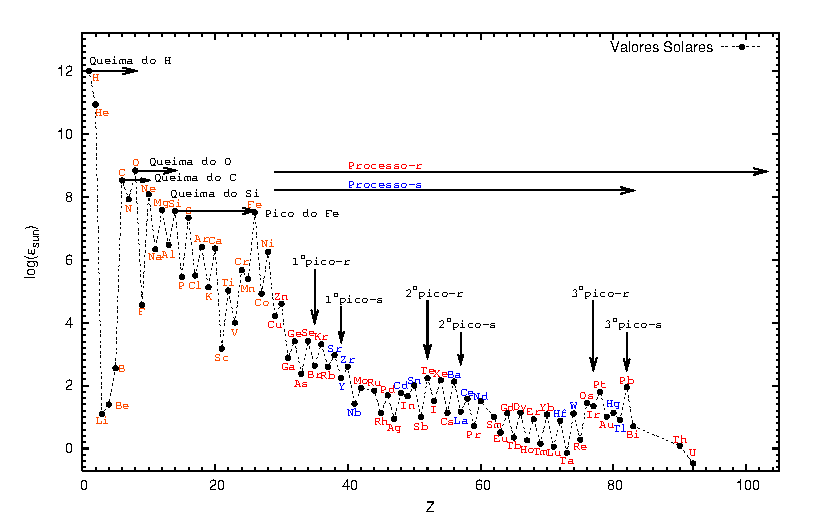
\includegraphics[width=1.0 \columnwidth,angle=0]{fig/solar_grevesse.eps}
\caption{Legenda da figura.} 
\label{identificador}
\end{center}
\end{figure}


\begin{center}
\setcaptionmargin{1cm}
\scriptsize
\begin{longtable}{lcccc}
\caption[Resumo da legenda da tabela (aparece na lista de figuras)]{Exemplo de tabela feita com o longtable.}\\
\hline \hline \\[-2ex]
\multicolumn{1}{c}{Coluna1} &
\multicolumn{1}{c}{Coluna2} &
\multicolumn{1}{c}{Coluna3} &
\multicolumn{1}{c}{Coluna4} &
\multicolumn{1}{c}{Coluna5} 

\\[0.5ex] \hline
\\[-1.8ex]

\endfirsthead

\multicolumn{5}{c}{\footnotesize{{\slshape{{\tablename} \thetable{}}} - Continua��o}}\\[0.5ex]

\hline \hline\\[-2ex]

\multicolumn{1}{c}{Coluna1} &
\multicolumn{1}{c}{Coluna2} &
\multicolumn{1}{c}{Coluna3} &
\multicolumn{1}{c}{Coluna4} &
\multicolumn{1}{c}{Coluna5} 

\\[0.5ex] \hline
\\[-1.8ex]

\endhead

\multicolumn{3}{l}{{\footnotesize{Continua na pr�xima p�gina\ldots}}}\\
\endfoot
\hline

\endlastfoot

1 & 2 & 3 & 4 & 5 \\
6 & 7 & 8 & 9 & 10\\

\label{tabela_com_longtable}
\end{longtable}
\end{center}


  	      					%
%% 										%
\bibliography{tex/bibliografia}					% referencias com bibTeX
										%
										%
\end{document}								% fim do documento
